\documentclass{article}
\usepackage[utf8]{inputenc}
\usepackage[T1]{fontenc}
\usepackage[french]{babel}

% ------------------------- Color table ----------------------------------------
\usepackage{multirow}
\usepackage[table]{xcolor}
\definecolor{maroon}{cmyk}{0,0.87,0.68,0.32}
% ------------------------------------------------------------------------------

\usepackage{amscd}
\usepackage{amsthm}
\usepackage{physics}
\usepackage[left=2.2cm,right=2.2cm,top=2cm,bottom=2cm]{geometry}
\usepackage{textcomp,gensymb} %pour le °C, et textcomp pour éviter les warning
\usepackage{graphicx} %pour les images
\usepackage{caption}
\usepackage{subcaption}
\usepackage[colorlinks=true,
	breaklinks=true,
	citecolor=blue,
	linkcolor=blue,
	urlcolor=blue]{hyperref} % pour insérer des liens
\usepackage{epstopdf} %converting to PDF
\usepackage[export]{adjustbox} %for large figures

\usepackage{array}
\usepackage{dsfont}% indicatrice : \mathds{1}


% -------------------------- Mathematics ---------------------------------------
\graphicspath{{images/}{../images/}} % For the images path
% ------------------------------------------------------------------------------

% -------------------------- Mathematics ---------------------------------------
\usepackage{mathrsfs, amsmath, amsfonts, amssymb}
\usepackage{bm}
\usepackage{mathtools}
\usepackage[Symbol]{upgreek} % For pi \uppi different from /pi
\newcommand{\R}{\mathbb{R}} % For Real space

% ------------------------------------------------------------------------------


% -------------------------- Code format ---------------------------------------
\usepackage[numbered,framed]{matlab-prettifier}
\lstset{
	style              = Matlab-editor,
	basicstyle         = \mlttfamily,
	escapechar         = '',
	mlshowsectionrules = true,
}
% ------------------------------------------------------------------------------

% ------------------------- Blbiographie --------------------------------------
\usepackage[backend=biber, style=ieee]{biblatex}
\addbibresource{biblio.bib}
% ------------------------------------------------------------------------------


\setcounter{tocdepth}{4} %Count paragraph
\setcounter{secnumdepth}{4} %Count paragraph
\usepackage{float}

\usepackage{graphicx} % for graphicspath
% \graphicspath{{../images/}}

\usepackage{array,tabularx}
\newcolumntype{L}[1]{>{\raggedright\let\newline\\\arraybackslash\hspace{0pt}}m{#1}}
\newcolumntype{C}[1]{>{\centering\let\newline\\\arraybackslash\hspace{0pt}}m{#1}}
\newcolumntype{R}[1]{>{\raggedleft\let\newline\\\arraybackslash\hspace{0pt}}m{#1}}

% to start counting section to 6


%%%%%%%%%%%%%%%%%%%%%%%%%%%%%%%%%%%%%%%%%%%
% Header
%%%%%%%%%%%%%%%%%%%%%%%%%%%%%%%%%%%%%%%%%%%

\renewcommand{\assignmenttitle}{Assignment 3 : Neural Networks}
\renewcommand{\studentname}{Vincent Matthys}
\renewcommand{\email}{vincent.matthys@ens-paris-saclay.fr}

% renew (sub)section to get alpanumeric characters
\renewcommand{\thesection}{\Roman{part}.\arabic{section}}

\usepackage{xpatch}

\xpretocmd{\part}{\setcounter{section}{0}}{}{}


%%%%%%%%%%%%%%%%%%%%%%%%%%%%%%%%%%%%%%%%%%%
% Syntax for using figure macros:
%%%%%%%%%%%%%%%%%%%%%%%%%%%%%%%%%%%%%%%%%%%

% \singlefig{filename}{scalefactor}{caption}{label}
% \doublefig{\subfig{filename}{scalefactor}{subcaption}{sublabel}}
%           {\subfig{filename}{scalefactor}{subcaption}{sublabel}}
%           {global caption}{label}
% \triplefig{\subfig{filename}{scalefactor}{subcaption}{sublabel}}
%           {\subfig{filename}{scalefactor}{subcaption}{sublabel}}
%           {\subfig{filename}{scalefactor}{subcaption}{sublabel}}
%           {global caption}{label}
%
% Tips:
% - with scalefactor=1, a single figure will take the whole page width; a double figure, half page width; and a triple figure, a third of the page width
% - image files should be placed in the image folder
% - no need to put image extension to include the image
% - for vector graphics (plots), pdf figures are suggested
% - for images, jpg/png are suggested
% - labels can be left empty {}

%%%%%%%%%%%%%%%%%%%%%%%%%%%%%%%%%%%%%%%%%%%
% Beginning of assignment
%%%%%%%%%%%%%%%%%%%%%%%%%%%%%%%%%%%%%%%%%%%
\begin{document}
\maketitle

\part{Training a fully connected neural network}


\part{CNN building blocks}

The gradient computations have been done in the \textit{gradient\_nn.m} file

\section{Convolution}

\question{2.3: \begin{enumerate}
		\item What filter have we implemented?
		\item How are the RGB colour channels processed by this filter?
		\item What image structure are detected?
	\end{enumerate}}
\begin{enumerate}
	\item The filter implemented is used to compute the Laplacian of the image
	\item Repeating the same filter over the 3 channels, the channells are processed with the same filter.
	\item The Laplacian kernel detects rapid changes in each color channel. To high response values correspond edges in general.
\end{enumerate}


\section{Non-linear activation functions}

\question{2.2: Some of the functions in a CNN must be non-linear. Why?}

With 0 non-linear functions, the CNN is equivalent to anoter CNN with larger convolutional kernels (resulting of the convolution of filters). Therefore it loses the capability of modeling more complex functions.

\section{Pooling}

\question{2.3: Look at the resulting image. Can you interpret the result?}
The resulting image is smaller, because of the lack of padding value (has to be set to 7 to keep the initial resolution for a 15x15 window). Moreover, the resulting image presents larger and blurred fruits. This is explained by the maximal value taken for each channel for each pixel.


\part{Back-propagation and derivatives}

\section{The theory of back-propagation}

\question{3.1.A: The derivatives \(\frac{\partial f}{\partial w_l}(x_0;w_1,…,w_L)\) (derivatives of the loss with respect to any parameters \(w_l\)) have the same size as the parameters \(w_l\). Why?}

The loss \(f\) is a scalar function, therefore taking its derivate w.r.t. any matrix is the same as taking the matrix composed with the derivative of \(f\) w.r.t. each element of the matrix. Consequently the derivatives \(\frac{\partial f}{\partial w_l}(x_0;w_1,…,w_L)\) has the same size as the parameters \(w_l\).

\part{Learning a character CNN}

\section{Prepare the data}

\section{Intialize a CNN architecture}

\question{4.2.A: By inspecting \textit{initializeCharacterCNN.m} get a sense of the architecture that will be trained. How many layers are there? How big are the filters?
}

There are 8 layers :
\begin{enumerate}
	\item convolution, with 20 filters 5x5
	\item spatial pooling, with 2x2 window
	\item convolution, with 50 filters 5x5
	\item spatial pooling, with 2x2 window
	\item convolution, with 500 filters 4x4
	\item non-linearity
	\item convolution, with 26 filters 2x2
	\item softmax loss layer
\end{enumerate}

\question{4.2.B: \begin{enumerate}
		\item Understand what the softmax operator does. Hint: to use the log-loss the data must be in the (0, 1] interval.
		\item Understand what is the effect of minimising the log-loss. Which neuron’s output should become larger?
	\end{enumerate}}

\begin{enumerate}
	\item The softmax operator (\(y_{ijk^{\prime}}\)) assign a probability for each spatial location \((i,j)\) to belong to class \(k^{\prime}\). Consequently the log of such computed probability can be computed.
	\item Minimizing the log-loss is training the soft-max model. The output of the neuron corresponding to the true class label should become larger.
\end{enumerate}

\section{Train and evaluate the CNN}

\question{4.3: Run the learning code and examine the plots that are produced. As training completes answer the following questions:
	\begin{enumerate}
		\item There are two sets of curves: energy and prediction error. What do you think is the difference? What is the "energy"?
		\item Some curves are labelled "train" and some other "val". Should they be equal? Which one should be lower than the other?
		\item Both the top-1 and top-5 prediction errors are plotted. What do they mean? What is the difference?
	\end{enumerate}}

\begin{enumerate}
	\item The energy curve represents the evolution of the network over time, \textit{e.g.} how the weights are varying. On the other hand the prediction error compares the true label with the top scoring labels returned by the network.
	\item The train curve represents the error on the training data, whereas the validation curve represents the error on the unseen data. The training error should therefore be lower than the other, as the network is learning how to minimize this precise error.
	\item In the top-1 prediction, we are looking if the true label is the one giving the maximal probability, as returned by the network. In the top-5 prediction, we look at the first 5 scoring classes and look if the true label class is one of them. It's clear that the top-5 prediction error is always smaller than the top-1, as being part of the 5 first scores not as hard as being the top scoring class.
\end{enumerate}

\section{Visualise the learned filters}

\question{4.4: what can you say about the filters?}

The filters from the first layers are hard to interpret. We can guess a dominance in term of response in the diagonals of the filters learnt

\section{Apply the model}

\question{4.5.A: The image is much wider than 32 pixels. Why can you apply to it the CNN learned before for 32x32 patches? Hint: examine the size of the CNN output using size(res(end).x).}

The CNN output size is \((1, 137, 26\)) which suppose that patches 32x32 from initial images have been taken, and the current CNN output a map of response of those 32x32 patches.

\question{4.5.B: Comment on the quality of the recognition. Does this match your expectation given the recognition rate in your validation set (as reported by cnn\_train during training)?}

The recognition is pretty bad. Not even a word is recognized. It's surprising because the traing error is below \(10~\%\). A possible explaination is the training context, where the network doesn't learn to recognize letters inbetween others.

\section{Training with jitter}

\question{4.6:
	\begin{enumerate}
		\item Look at the training and validation errors. Is their gap as wide as it was before?
		\item Use the new model to recognise the characters in the sentence by repeating the previous part. Does it work better?
	\end{enumerate}}

\begin{enumerate}
	\item
	\item The recognition of the characters is almost perfect, if we can forget the repetition of the characters because of the stride chosen by the network.
\end{enumerate}

% \part{Using pretrained models}
%
% \section{Image classification with a pretrained CNN}
%
% \question{5.1:
% 	\begin{enumerate}
% 		\item Show the classification result.
% 		\item List the top-5 classes
% 	\end{enumerate}}
%
% \begin{figure}[ht!]
% 	\centering
% 	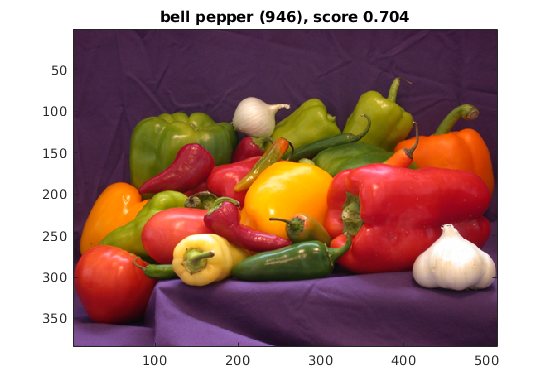
\includegraphics[height = 0.5\textheight]{5_1.png}
% 	\caption{Classification results of peppers}
% 	\label{fig_5_1}
% \end{figure}
%
% \begin{enumerate}
% 	\item Le résultat de la classification est présenté en figure~\ref{fig_5_1}.
% 	\item Les 5 premières classes sont
% \end{enumerate}
%
% \section{Image classification using CNN features and linear SVM}


\end{document}
